\documentclass[main.tex]{subfiles}

\begin{document}

% \textcolor{red}{Вводная лекция}

\section{Лекция 09.03.2021 (Донцов Е.В.)}

\subsection{Математическая модель полубесконечной трещины ГРП. Продолжение}

\includegraphics[width=\textwidth, page=30]{HF_slides_2021.pdf}

Я доработал вывод уравнений для модели полубесконечной трещины, поэтому давайте ещё раз его вспомним.
\\

Трудно сразу провести анализ полученной нами системы уравнений для модели плоской трещины.
Поэтому (чтобы понять происходящее) рассмотрим более простую задачу о полубесконечной трещине.
Это самая простая геометрия и для неё легче всего найти решение.

Что такое полубесконечная трещина?
Зачем она нужна?

Если рассмотрим задачу о плоской трещине и приблизимся к кончику трещины (т.е. мы хотим понять, что происходит возле границы трещины, когда она распространяется), то как раз получим геометрию полубесконечной трещины.
Понятно, что ничего полубесконечного в жизни не бывает, это некая математическая идеология, но необходимо понимать, что физически мы рассматриваем проблему возле кончика трещины.

Основные (изначальные) уравнения соответствуют плоской трещине.
Далее, чтобы перейти к полубесконечной трещине, мы рассматриваем проблему, в которой рассматриваемая трещина едет (распространяется) с некой постоянной скоростью $V$.

Вводим движущуюся систему координат (начало координат находится в кончике трещины, ось $O\hat{x}$ направлена внутрь трещины):
\beq
\hat{x}=Vt-x
\eeq

Предполагаем, что в этой системе координат задача стационарная, т.е. вся зависимость от времени зашита в $\hat{x}$ (нет ещё отдельной дополнительной зависимости от времени).

Тогда уравнение
\beq
\frac{\partial w}{\partial t}+\frac{\partial q}{\partial x}+\frac{C'}{\sqrt{t-t_0(x)}}=Q_{0,ps}(t)\delta(x)
\eeq
перепишется в виде обыкновенного дифференциального уравнения:
\beq
V\frac{dw}{d\hat{x}}-\frac{dq}{d\hat{x}}+\frac{C'}{\sqrt{\hat{x}/V}}=0
\eeq

Далее интегрируем полученное уравнение по $\hat{x}$:
\beq
\frac{w^2}{\mu'}\frac{dp}{d\hat{x}}=V+2C'\frac{\sqrt{V\hat{x}}}{w}
\eeq
(здесь учли, что $q=-\dfrac{w^3}{\mu'}\dfrac{\partial p}{\partial x}$).

Далее следующий шаг упрощения задачи: вместо прямого уравнения упругости используем обратное уравнение упругости, в котором открытие будет функцией градиента давления.
Самое главное, что в этой формулировке мы автоматически удовлетворяем критерию распространения.
Открытие будет равно некой корневой зависимости (т.е. это и есть критерий распространения) плюс некое слагаемое, зависящее от градиента давления.

Если интересно: все эти функции считаются через преобразование Фурье.
В Фурье-образах интегральное уравнение превращается в очень простое соотношение между давлением и открытием.

Итог: у нас было 4 уравнения (закон сохранения объёма, связь потока с градиентом давления, упругость и критерий распространения); после всех математических манипуляций остались только 2 уравнения.

\includegraphics[width=\textwidth, page=31]{HF_slides_2021.pdf}

Далее рассмотрим некий математический трюк, с помощью которого из оставшихся двух уравнений сделаем только одно уравнение.

Получили одно интегральное уравнение на открытие, в котором присутствуют все входные параметры задачи.

Далее производим масштабирование (обезразмеривание), т.е. вводим безразмерные переменные.
Идея в том, что после того, как мы отмасштабируем уравнение, мы получим очень простое безразмерное уравнение в представленной на слайде форме.

Фактически получили уравнение на одно безразмерное открытие $\tilde{w}$.

Важно то, что в полученном уравнении нет сингулярностей.

\includegraphics[width=\textwidth, page=32]{HF_slides_2021.pdf}

Итак, мы пришли к одному уравнению на безразмерное открытие, в котором есть 3 характерных слагаемых: первое (внеинтегральное) слагаемое описывает эффект трещиностойкости, второе слагаемое включает в себя эффект вязкости, третье слагаемое отвечает за утечки.

Соответственно выделяют 3 аналитических решения:

1) в случае доминирования трещиностойкости (при очень маленьких вязкости и утечках, например, закачиваем воду в практически непроницаемый резервуар);

2) в случае доминирования вязкости (чтобы трещиностойкость была пренебрежимо малой, можно представить себе, что мы закачиваем жидкость в уже существующую трещину) -- получается некое интегральное уравнение -- на следующем слайде будет представлено полное решение этого уравнения;

3) в случае доминирования утечек.

\includegraphics[width=\textwidth, page=33]{HF_slides_2021.pdf}

Теперь покажу вывод решения в случае доминирования вязкости.

Предполагаем решение в форме степенной функции, подставляем и находим константы (интеграл считается аналитически).

\includegraphics[width=\textwidth, page=34]{HF_slides_2021.pdf}

Теперь посмотрим, как выглядит полное решение.
Можем его найти численно.

На центральном графике на слайде: чёрная линия -- численное решение рассматриваемого интегрального уравнения (при некотором наборе входных параметров), цветными линиями показаны предельные аналитические решения.

Видим, что по порядку величины не ошибёмся, если возьмём максимум известных аналитических решений.

\includegraphics[width=\textwidth, page=23]{HF_slides_2022.pdf}

Повторюсь, что даже в приближении решения в виде максимума предельных решений будет относительно неплохой ответ (он будет негладкий, но он будет вполне точный).

Но давайте выведем гладкое и ещё более точное приближённое решение.

Для этого:

1) дифференцируем интегральное уравнение;

2) предполагаем, что безразмерное открытие пропорционально некой степени безразмерной координаты $\tilde{x}$ (мы же видели, что все предельные решения имеют степенной характер зависимости от координаты);

3) заменяем функцию $G'$ дельта-функцией (если нарисуем график функции $G'$, то увидим, что она очень похожа на дельта-функцию) -- здесь ещё важно, что выражение в квадратных скобках меняется слабо, так как мы предполагаем, что $\delta$ меняется слабо (от 0 до 1/3 -- оно не меняется на порядки).
\\

Важно, что в итоге получается некое дифференциальное уравнение, в котором $C_1$ и $C_2$ слабо меняются в зависимости от $\delta$.

\includegraphics[width=\textwidth, page=36]{HF_slides_2021.pdf}

Из верхних графиков на слайде видим, что $C_1$ и $C_2$ слабо изменяются в зависимости от $\delta$.
Т.е. даже если примем $C_1$ и $C_2$ за константы, то всё равно с хорошей точностью опишем решение.
Так и сделаем.

Получим неявную зависимость открытия $\tilde{w}_0$ от $\tilde{x}$ и $\chi$.
И это общая форма решения во всём параметрическом пространстве.

Далее можно пересчитать $\delta$ на основе полученного решения, подставить его в уравнение и найти следующее приближение к решению.

Первое приближение даёт максимальную погрешность в 1 процент (по сравнению с численным решением), а второе приближение даёт максимальную погрешность в 0.14 процента.
Это погрешность между только что полученным приближённым полуаналитическим решением и численным решением во всём параметрическом пространстве.

Таким образом, получили хорошее полуаналитическое приближение для полного решения полубесконечной трещины.

\includegraphics[width=\textwidth, page=37]{HF_slides_2021.pdf}

На этом мы заканчиваем раздел про полубесконечную трещину.

Я хочу, чтобы вы запомнили, что полубесконечная трещина -- это модель трещины ГРП, которая описывает кончик конечной трещины (плоской, планарной и т.п.).

Для полубесконечной трещины существует 3 предельных аналитических решения (доминирование трещиностойкости, вязкости или утечек), которые представляют из себя некие степенные функции, показывающие характер зависимости раскрытия от расстояния от кончика трещины и всех входных параметров задачи.

Полное решение модели полубесконечной трещины плавно переходит от одного предельного решения к другому.

Если на пальцах необходимо посчитать полное решение, то можно взять максимум между предельными аналитическими решениями (и тем самым оценить открытие в зависимости от входных параметров задачи).

Получено приближённое решение для полного решения задачи о полубесконечной трещине.
Это приближённое решение может быть использовано в качестве условия распространения в численных моделях расчёта ГРП.

\subsection{Математическая модель плоской трещины ГРП. Продолжение}

\includegraphics[width=\textwidth, page=38]{HF_slides_2021.pdf}

Давайте обсудим (проведём анализ) плоской трещины (двухмерная упругость, одномерное течение) более подробно.

Ранее изучили более простую модель полубесконечной трещины и для неё выяснили, что в определённых предельных случаях можем посчитать точное аналитическое решение, а полное решение задачи получается приближённым (с ошибкой примерно 0.1 процента).
Т.е. для полубесконечной трещины не можем абсолютно точно найти полное решение.

Для плоской трещины ситуация будет очень похожая: в каких-то приближениях (предельных случаях) мы сможем найти точное решение.
А полное решение можно будет тоже построить (состряпать) из предельных решений, но оно будет приближённым.
\\

Ещё раз напомню проблему: есть одномерная трещина, которая распространяется в упругом материале (в условиях плоских деформаций), закачиваем жидкость с определённым расходом $Q_0$, есть входные параметры (вязкость, утечеки, трещиностойкость, модуль Юнга), мы хотим посчитать открытие как функцию времени и координаты.

Сделаем некий математический трюк (масштабирование / обезразмеривание).
Давайте посмотрим, в каких пределах по порядку величины меняются слагаемые в рассматриваемых уравнениях.
В итоге, получаем алгебраическую систему уравнений на характерные масштабы рассматриваемых величин (обозначены индексом *).

Но видим, что в этой алгебраической системе 6 уравнений и 4 неизвестных.
Поэтому нет общего красивого решения.
Но если мы занулим некоторые параметры, то тогда сможем получить аналитическое решение (аналогичная ситуация была и для полубесконечной трещины).
Мы хотим 4 уравнения и 4 неизвестных, поэтому нужно занулить два каких-то параметра.
\\

Замечание: в постановке задачи в определяющих уравнениях нет сжимающего напряжения $\sigma_0$.
Т.е. на самом деле решение этой задачи по большей части не зависит от $\sigma_0$.
Это сжимающее напряжение сидит в определении коэффициента Картера (если $p_n$ много меньше, чем $\sigma_0$ минус поровое давление, то можно коэффициент Картера посчитать при $p=\sigma_0$).
Величина $p_n$ -- это так называемое чистое давление (net pressure), которое определяет, насколько преодолели давление $\sigma_0$ (чтобы раскрыть трещину).

В такой постановке важно, что $\sigma_0$ постоянно.

\includegraphics[width=\textwidth, page=39]{HF_slides_2021.pdf}

Рассмотрим предельное решение viscosity-storage, которое реализуется при доминировании вязкости (нет трещиностойкости и нет утечек).
Убираем два соответствующих уравнения и получаем 4 уравнения с четырьмя неизвестными.
Решаем полученную алгебраическую систему уравнений и находим выражения для характерных величин (зависимости от входных параметров задачи и времени).

Заметьте, что результат получили чисто из масштабирования и при этом не решали дифференциальные уравнения.
\\

Если найдём точное решение ($M$-vertex solution) для рассматриваемого режима (доминирование вязкости), то увидим, что оно представляет из себя некий числовой множитель умножить на только что найденный нами характерный масштаб и умножить на некоторую безразмерную функцию от безразмерной координаты $\xi$.

Видим, что открытие, полученное чисто из масштабирования (без решения дифференциальных уравнений) отличается от точного решения примерно на 13 процентов.

\includegraphics[width=\textwidth, page=40]{HF_slides_2021.pdf}

Рассмотрим предельный случай toughness-storage, который реализуется при доминировании трещиностойкости (нет вязкости и нет утечек).
Убираем два соответствующих уравнения и получаем 4 уравнения с четырьмя неизвестными.
Решаем полученную алгебраическую систему уравнений и находим выражения для характерных величин (зависимости от входных параметров задачи и времени).

Заметьте, что результат получили чисто из масштабирования и при этом не решали дифференциальные уравнения.
\\

Если найдём точное решение ($K$-vertex solution) для рассматриваемого режима (доминирование трещиностойкости), то увидим, что оно представляет из себя некий числовой множитель умножить на только что найденный нами характерный масштаб и умножить на некоторую безразмерную функцию от безразмерной координаты $\xi$.

Видим, что открытие, полученное чисто из масштабирования (без решения дифференциальных уравнений) отличается от точного решения примерно на 30 процентов.
\\

Обратите внимание, что при доминировании трещиностойкости давление не зависит от координаты, т.к. нет вязкости.

Примечание: давление падает только тогда, когда есть вязкость;
именно из-за вязкости возникает трение, которое необходимо преодолеть, и соответственно появляется падение давления из-за трения;
а если нет вязкости, то нет и градиента давления, поэтому давление не зависит от координаты.

\includegraphics[width=\textwidth, page=41]{HF_slides_2021.pdf}

Теперь давайте рассмотрим качественный переход между трещиностойкостью и вязкостью.

На примере полубесконечной трещины видели, что есть несколько предельных степенных решения, а общее решение плавно переходит от одного предельного решения к другому.

Для полубесконечной трещины переход происходил при увеличении расстояния от кончика трещины.

А здесь (в рассматриваемой задаче о плоской трещине) переход между режимами будет происходить с течением времени (решение будет плавно переходить от одной функции к другой функции).

Чтобы определить, какой параметр отвечает за этот переход, берём решение для масштабов длин (или открытий, или давлений) в двух режимах и приравниваем их.
Получаем безразмерную трещиностойкость.
Этот параметр определяет, насколько большая трещиностойкость.

Если безразмерная трещиностойкость много меньше единицы, то эффект трещиностойкости много меньше эффекта вязкости ($M$ vertex solution).

Если безразмерная трещиностойкость много больше единицы, то эффект трещиностойкости будет доминировать (вязкость будет мала по сравнению с трещиностойкостью; $K$ vertex solution).

Ясно, что мы не можем просто сравнить вязкость и трещиностойкость (хотя бы потому что у них разные размерности), поэтому необходимо проводить анализ в безразмерных переменных.
\\

Но рассмотрели ещё только первую часть, так как рассматривали предельные решения и переход между ними в случае отсутствия утечек.

\includegraphics[width=\textwidth, page=42]{HF_slides_2021.pdf}

В общем и целом для конечной плоской трещины есть соревнование на доминирование между трещиностойкостью и вязкостью (эти два процесса создают сопротивление росту трещины и отвечают за диссипацию);
и дополнительно есть характеристика утечек (бОльшая часть жидкости остаётся в трещине или же бОльшая часть жидкости утекает в породу).

Соответственно получаем 4 предельных решения:

1) доминирующая вязкость и маленькие утечки (режим $M$ -- storage-viscosity);

2) доминирующая вязкость и большие утечки (режим $\tilde{M}$ -- leak-off-viscosity);

3) доминирующая трещиностойкость и маленькие утечки (режим $K$ -- storage-toughness);

4) доминирующая трещиностойкость и большие утечки (режим $\tilde{K}$ -- leak-off-toughness).

Это довольно большое отличие от полубесконечной трещины (для неё было только 3 предельных решения).
\\

Замечание: 4 предельных режима будут не только в случае плоской трещины, но и для радиальной трещины, и для PKN модели.

\includegraphics[width=\textwidth, page=43]{HF_slides_2021.pdf}

Важно знать связь между предельными решениями для плоской конечной трещины и предельными решениями для полубесконечной трещины.
Вопрос стоит так: задан предельный режим распространения плоской трещины, необходимо определить какой режим реализуется возле кончика.
\\

Вязкостная асимптота на кончике соответствует решению $M$ (режим storage-viscosity) плоской трещины.
Другими словами, когда плоская конечная трещина распространяется в предельном режиме большой вязкости и малых утечек, то возле кончика поведение будет описываться вязкостной асимптотой решения для полубесконечной трещины.
\\

Появляется некая неоднозначность с трещиностойкостью: если доминирует трещиностойкость, то не важна интенсивность утечек, на кончике всегда открытие ведёт себя как корень из $\hat{x}$, т.е. для двух предельных решений плоской трещины одна и та же асимптота на кончике.

Но хочу обратить внимание, что решение вдали от кончика всё равно разное, например, в storage-toughness объём трещины будет больше, чем в leak-off-toughness (при одинаковой скорости закачки), так как в режиме storage-toughness нет утечек.
Но поведение возле кончика в режимах storage-toughness и  leak-off-toughness одинаковое.

Вообще это достаточно интересно, что асимптотика трещиностойкости реализуется на двух предельных решениях модели плоской трещины.
\\

В предельном режиме большой вязкости и больших утечек плоской трещины (leak-off-viscosity) на кончике этой трещины реализуется асимптотический режим утечек полубесконечной трещины.
\\

Дальше пойдём в большие глухие дебри.
Расскажу больше про предельные режимы модели плоской трещины, при каких параметрах реализуются эти режимы, где найти решения для всех этих предельных режимов и как построить приближённое решение, которое описывает все 4 предельных случая и переходы между ними.

Домашние задания по выводу формул на самом деле сложно сделать сходу; есть много технических деталей.

\includegraphics[width=\textwidth, page=44]{HF_slides_2021.pdf}

Далее давайте поговорим про численное и приближённое аналитическое  решения в общем случае.

Ранее поговорили о том, как можно на пальцах оценить решение, но понятно, что полностью точно решить систему уравнений модели плоской трещины аналитически практически невозможно (т.к. в нём есть дифференцальное уравнение в частных производных + интегральное уравнение + нелинейности + подвижные границы).

Один из основных методов решения такой системы -- это метод численного решения.
Но также можно найти приближённое аналитическое решение.
\\

Численное решение: берём систему уравнений, дискретизируем её с помощью метода конечных разностей и после этого решаем дискретную систему уравнений.
Этот метод применим к любому типу уравнений (и в рассматриваемом случае тоже), но мы не будем заморачиваться на деталях численной реализации.
\\

Я хочу рассказать вам, как качественно построить приближённое решение и почему оно работает.

Зачем мы хотим построить приближённое решение?
Хотим качественно понять и уловить основные моменты решения, чтобы более точно описать процесс распространения трещины.

На графике на слайде я привожу пример раскрытия плоской трещины как функцию координаты $x$.
Численное решение показано квадратными маркерами.
Если нарисуем асимптотическое решение возле кончика, то оно будет выглядеть подобно синей линии.
Возле кончика асимптотическое решение всегда (при любых значениях входных параметров) будет совпадать с решением плоской трещины.
В этом и есть суть асимптотики.
Мы знаем приближённое асимптотическое решение на кончике для всех режимов (значений входных параметров модели).

Недавно я заметил, что если домножить это асимптотическое решение на $\sqrt{\frac{1}{2}\left(1+x/l\right)}$, то полученное решение будет очень хорошо совпадать с численным решением.

Откуда берётся этот множитель?

Для решения, которое соответствует режиму трещиностойкости, мы знаем аналитическое решение для открытия (это будет просто эллипс) и мы знаем аналитическое решение для асимптотики (это будет корень).
Далее просто берём отношение одного решения к другому и получаем множитель.

Для режимов $K$ и $\tilde{K}$ этот множитель точен, а для решения с доминирующей вязкостью этот множитель приблизителен, но тем не менее он описывает 90-95\% всего решения и поэтому его можно использовать.
\\

Но это же не полное решение, для полного решения необходимо найти длину от времени, открытие от времени и т.д.
Чтобы это всё найти мы используем только что найденную форму решения для открытия как функцию координаты $x$ и подставляем её в общий закон сохранения объёма.
Получаем 2 уравнения с двумя неизвестными, которые решаются численно, но без использования полной численной схемы (решаются очень быстро).
В режиме трещиностойкости параметр $\lambda=1/2$, а при других (более нетривиальных) режимах мы этот параметр подгоняем под численное решение.
При этом $\lambda$ для разных режимов варьируется слабо.
Но вообще лямбду отличную от одной второй используем, если хотим увеличить точность (например, уменьшить погрешность с 5\% до 1\%).

Зачем это надо?
Чтобы построить карту режимов...

\includegraphics[width=\textwidth, page=45]{HF_slides_2021.pdf}

Ранее обсуждали, как получить безразмерную трещинстойкость $K_m$.
Аналогичным образом можем получить безразмерное время (оно нормируется на величину, представленную на слайде).
\\

Используя полуаналитическое приближённое решение, можно найти решение во всём параметрическом пространстве очень быстро (примерно за 1 час).

Численное решение тоже можно было использовать, но тогда количество точек в параметрическом пространстве, на которых производился бы расчёт, пришлось бы уменьшить.
Плюс это всё решалось бы несколько недель, нужно было бы организовать распараллеливание.

В общем, приближённым полуаналитическим решением построить карту режимов в разы удобнее.

И в итоге мы можем построить зоны применимости всех предельных решений.
\\

Замечание: численное решение часто начинает разваливаться или сильно замедляется (требует очень маленький шаг по времени) при очень высоких утечках; у приближённого полуаналитического решения таких проблем нет.
\\

На карте режимов цветом показано безразмерное открытие как функция двух безразмерных параметров ($K_m$ и $\tau$).

Видим, что полное решение плавно перетекает от одного предельного режима к другому (похожая ситуация была и для модели полубесконечной трещины).
\\

Замечание. Есть такая особенность, что из $M$ режима вы не сможете попасть в режим $\tilde{K}$ с течением времени (при неизменных остальных входных параметрах модели);
из $M$ режима вы можете попасть в режим $\tilde{M}$ с течением времени.
Это связано с тем, что по оси абсцисс на карте режимов отложено время, а безразмерная трещиностойкость (отложенная по оси ординат) зафиксирована.

Это одно из важных свойств рассматриваемой модели плоской трещины, и не у всех моделей ГРП есть такое свойство.

\includegraphics[width=\textwidth, page=46]{HF_slides_2021.pdf}

Для всех четырёх предельных режимов плоской трещины есть явные аналитические формулы для открытия, давления и длины трещины (в виде функций координаты и времени, а также входных параметров модели).

Аналогично модели полубесконечной трещины при необходимости знать полное решение модели плоской трещины можно воспользоваться максимумом (или минимумом) из всех предельных решений.
С помощью такого подхода можно оценить длину трещины, давление и открытие на пальцах (например, при проведении лабораторного эксперимента).

\includegraphics[width=\textwidth, page=47]{HF_slides_2021.pdf}

Здесь представлено много графиков.

Давайте я акцентирую внимание на нескольких из них.
Из левых четырёх графиков можем увидеть сильную разницу между режимами трещиностойкости ($K_m=6$) и вязкости ($K_m=0.5$).
Давление вдоль трещины в режиме трещиностойкости постоянно, а в режиме доминирования вязкости давление существенно изменяется вдоль трещины.
\\

$\xi$ -- безразмерная координата;
$\Omega$ -- безразмерное открытие;
$\Pi$ -- безразмерное давление;
$\gamma$ -- безразмерная длина;
$\eta$ -- эффективность (определяет утечки; если равна 1, то вся закачанная жидкость осталась в трещине; если равна 0, то вся жидкость утекла из трещины)
\\

Все величины на графиках (открытие, давление и длина) нормированы на соответствующие вязкостные решения без утечек для соответствующих величин.

\includegraphics[width=\textwidth, page=48]{HF_slides_2021.pdf}

На этом мы заканчиваем раздел про плоскую трещину.
В этом разделе на самом деле есть очень много технических деталей, которые я специально опустил.

Ранее (ещё до подробного разбора модели плоской трещины) мы прошлись по техническим деталям вывода базовых уравнений моделей трещины ГРП, по техническим деталям вывода решений для полубесконечной трещины.

Чем сложнее становится геометрия, тем насыщеннее становится математика.
\\

Но я думаю, что здесь наиболее важно понимание физики и понимание того, какие предельные решения существуют, в чём их смысл, как они переходят друг в друга и как их использовать.
\\

Для плоской трещины решаем двухмерное уравнение упругости и одномерное уравнение течения.

Мы оценили решение, исходя из оценки масштабов слагаемых в системе уравнений (смогли оценить решение в предельных случаях с точностью до численного множителя).

Важно помнить связь между предельными режимами плоской трещины и асимптотиками возле кончика трещины.
\\

Для плоской трещины существует приближённое полуаналитическое решение.

Также существуют точные аналитические решения для четырёх предельных режимов.
Их важно знать, например, если вы написали свой численный алгоритм для трещины ГРП и хотите его проверить.
Важно делать проверку в разных режимах, так как, например, только в режиме $K$ не сможем проверить правильность имплементации вязкостных эффектов.
\\

Важно, что для модели плоской трещины существует параметрическое пространство, которое можно реконструировать, используя, например, полученные приближённые полуаналитические решения.

\end{document}
